\documentclass[12pt]{article}

\usepackage[utf8]{inputenc}
\usepackage{latexsym,amsfonts,amssymb,amsthm,amsmath}
\usepackage{tikz}
\usepackage{stanli}
\usetikzlibrary{shapes,calc,through,3d,patterns}
\usetikzlibrary{arrows.meta,decorations.pathreplacing,angles,quotes}
\usepackage{multicol}
\usepackage{geometry}
\usepackage{mathtools}
\usepackage{siunitx}
\usepackage{booktabs}
\usepackage{tabularx}


\setlength{\parindent}{0in}
\setlength{\oddsidemargin}{-0.25in}
\setlength{\textwidth}{7in}
\setlength{\textheight}{9.3in}
\setlength{\topmargin}{-1in}
\setlength{\headheight}{18pt}

\newcommand\blfootnote[1]{%
    \begingroup
    \renewcommand\thefootnote{}\footnote{#1}%
    \addtocounter{footnote}{-1}%
    \endgroup
}

\definecolor{darkred}{rgb}{0.6,0,0}

\newcommand{\bolddelta}{\boldsymbol\delta}
\newcommand{\boldxi}{\boldsymbol\xi}

\newcolumntype{M}[1]{>{\centering\arraybackslash}m{#1}}


\begin{document}

\noindent
\begin{minipage}[b]{320pt}
	\begin{flushleft}
		\textbf{ME-473}\\
		\textbf{Dynamic finite element analysis of structures}\\
		Stefano Burzio\\
		2024-2025
	\end{flushleft}
\end{minipage}
\hfill
\begin{minipage}[b]{80pt}
	\begin{flushright}
		
\includegraphics[scale=0.6]{../images/epfl-logo.pdf}
		\vspace{0.3cm}
	\end{flushright}
\end{minipage}

\vspace{0.5cm}
\hrulefill
\vspace{0.5cm}

\hspace*{\fill}\textbf{\Large Practice exam}\hspace*{\fill}

\hrulefill

\noindent
\begin{tabularx}{\textwidth}{p{6cm}r}
	\hline
	 &                                                                                                                                                             \\
	\multicolumn{2}{l}{First name : .............................................................................................................................} \\[15pt]
	\multicolumn{2}{l}{Last name : ..............................................................................................................................} \\
	[15pt]
	\multicolumn{2}{l}{SCIPER : .................................................................................................................................} \\
	\hline
\end{tabularx}


\noindent
\begin{center}
	\fbox{
		\parbox{160mm}{\centering
			\mbox{}
			\vspace{2mm}
			\begin{itemize}
				\setlength\itemsep{-1mm}
				\item Duration: 150 minutes.
				\item The exam is open book.
				\item Place your student ID card on the table.
				\item The use of a calculator is allowed.
				\item The use of any other electronic device is strictly prohibited during the exam.
			\end{itemize}
			\vspace{-1mm}
			\mbox{}

			\setlength{\tabcolsep}{18pt}
			\renewcommand{\arraystretch}{2}
			\begin{center}
				\begin{tabular}{@{} |l|M{6cm}| @{}}
					\hline
					Problem 1                     & \hspace{3cm}/ 25 points \\[10pt] \hline
					Problem 2                     & \hspace{3cm}/ 25 points \\[10pt] \hline
					\textbf{\emph{Sum of points}} & \hspace{3cm}/ 50 points \\[10pt] \hline
					\textbf{\emph{Final grade}}   &                         \\[10pt] \hline
				\end{tabular}
			\end{center}
		}
		\newline

	}
\end{center}
\newpage


\subsection*{Problem 1 {\small (25 points)}}
Consider a prismatic beam of length \( \ell \), constant cross-sectional area \( A \), flexural rigidity \( EI \), and mass density \( \rho \), undergoing transverse vibrations. The beam is modeled using Euler-Bernoulli beam theory, neglecting shear deformation and rotary inertia, and is clamped at both ends.\begin{center}
	\begin{tikzpicture}[scale=1]
		\point{a}{0}{0.5};
		\support {3}{a}[270];
		\point{b}{10}{0.5};
		\support {3}{b}[90];
		% Draw the rectangle
		\filldraw[fill=gray!40, draw=black,thick] (0,0) rectangle (10,1);
		%axis
		\draw[-latex, ultra thin] (0,0.5) -- (2,0.5) node[above]{$x$};
		\draw[ultra thin] (0,0.5) -- (10,0.5);
		\draw[-latex, ultra thin] (0,-0.5) -- (0,2) node[above]{$y$};
		% length
		\draw[ultra thin] (10,-0.5) -- (10, 2) ;
		\draw[latex-latex, ultra thin]  (0,1.5)  to node[sloped,midway,above] {$\ell$}(10,1.5) ;
		% Param
		\draw[ultra thin]  (7,0.3) -- (8,-1) node[right]{$E,A,\rho,I$};
	\end{tikzpicture}
\end{center}
The weak form of the governing equations of motion is given by:
\[
	\int_0^\ell EI\, \partial_{xx}^2 u_2 \, \partial_{xx}^2 \delta u_2 \, dx + \int_0^\ell \rho A\, \ddot u_2 \, \delta u_2 \, dx = 0,
\]
where \( u_2 \in \mathcal{U} \) denotes the transverse displacement field, and \( \delta u_2 \in \mathcal{V} \) is the corresponding virtual displacement.
\begin{itemize}
	\item[(a)] (3 points)  Provide the definition of the functional spaces \( \mathcal{U} \) and \( \mathcal{V} \).
	\item[(b)] (7 points) Derive the semi-discrete weak form by discretizing the domain using two Hermitian beam finite elements of equal length:
	      \begin{itemize}
		      \item Retrieve and assemble the elementary stiffness and consistent mass matrices.
		      \item Impose the essential boundary conditions to reduce the global system.
		      \item Explain the physical significance of each component in the generalized displacement vector \( \mathbf{q}(t) \), and identify the degrees of freedom associated with each node.
	      \end{itemize}
	\item[(c)] (6 points)  Formulate the generalized eigenvalue problem corresponding to the semi-discrete system obtained in part (b), and compute the two lowest natural frequencies and the associated mode shapes of the structure.
	\item[(d)] (4 points)  Explain whether the approximated natural frequencies are expected to be higher or lower than the exact ones.  Additionally, describe how the error may be quantified. If the number of elements is doubled, would you expect the computed fundamental frequency to increase or decrease compared to the value obtained with two finite elements? Provide justification for the following reasoning.

	\item[(e)] (5 points) To simplify the numerical computation, assume normalized parameters: \( E = A = \rho = I = \ell = 1 \). The beam is now subjected to a time-harmonic transverse point load of the form
	      \[
		      F(t) = A \sin(\bar\omega t)
	      \]
	      applied at the midpoint \( x = \ell/2 \), where \( A \) and \( \bar\omega \) are given constants. Assuming the beam is initially at rest with zero initial velocity, compute the transient response \( \mathbf{q}(t) \) for \( t\in]0,T[ \).
\end{itemize}

\subsection*{Problem 2 {\small (25 points)}}
We consider the problem of transverse vibrations of a homogeneous, isotropic  right-triangular membrane $\Omega$ under uniform tension which is supported along the edge parallel to the $y$-axis and spring-supported at the opposite vertex (3), as shown in the figure below.

\begin{center}
	\begin{tikzpicture}
		\point{a}{0}{0};
		\support {3}{a}[270];
		\point{b}{2}{2};
		\support {3}{b}[270];
		\point{c}{1}{1};
		\support {3}{c}[270];
		\point{d}{7}{2};
		\support {5}{d}[0];
		% Draw the rectangle (domain)
		\filldraw[fill=gray!40, draw=black,thick]  (0,0)-- (7,2) -- (2,2) -- cycle;
		% Labels for dimensions
		\draw[ultra thin] (0,0) -- (-0.7,-0.7);
		\draw[ultra thin] (2,2) -- (1,2);
		\draw[ultra thin] (7,2) -- (4.3,-0.7);
		\draw[ultra thin,latex-latex] (-0.7,-0.7) -- (4.3,-0.7) node[midway, below] {$1$};
		\draw[ultra thin,latex-latex] (-1,0) -- (1,2) node[midway, left] {$1$};
		% Axes
		\draw[ultra thin,-latex] (-1,0) -- (6,0) node[right] {$x$};
		\draw[ultra thin,-latex] (-.5,-0.5) -- (2.7,2.7) node[above] {$y$};
		% Arrows representing force p
		\draw[thick,-latex] (1.5,.6) -- (1.5,1.1);
		\draw[thick,-latex] (2.6,.95) -- (2.6,1.45);
		\draw[thick,-latex] (1.85,.95) -- (1.85,1.45);
		\draw[thick,-latex] (3,1.3) -- (3,1.8);
		\draw[thick,-latex] (4,1.3) -- (4,1.8);
		\draw[thick,-latex] (2.25,1.3) -- (2.25,1.8);
		\node at (3.5,2.3) {$\mathbf p$};
		% Labels
		\draw[ultra thin] (4.7,1.7) -- (7,3) node[right]{$S, \rho$};
		\draw[fill=white, draw=black] (0,0) circle (6pt) node{$1$};
		\draw[fill=white, draw=black] (7,2) circle (6pt) node{$2$};
		\draw[fill=white, draw=black] (2,2) circle (6pt) node{$3$};
	\end{tikzpicture}
\end{center}

The membrane has the following physical properties: mass density: $\rho = 1$ kg/m$^2$ and tension per unit length: $S = 2$ N/m. A uniform vertical pressure of magnitude $A = 3$ N/m$^2$ is applied over the entire triangle for 2 seconds. Thus $p(x, y, t) = A \theta(t)$ where
$$\theta(t)=\begin{cases}
		1 & \mbox{if } 0\leq t\leq 2 \\
		0 & \mbox{if } 1\leq t\leq T \\
	\end{cases}.$$
Moreover, the spring stiffness is $k = 10$ \text{N/m}.
\begin{itemize}
	\item[(a)] (5 points) Write the strong form and show that the weak form governing the transverse vibrations of the membrane is: find \( u_3 \in \mathcal{U} \) such that
	      \[
		      \int_{\Omega} \rho \, \ddot{u}_3 \, \delta u_3 \, d\Omega + \int_{\Omega} S \, (\nabla \delta u_3)^T\nabla u_3 \, d\Omega  + k u_3(1,1)\, \delta u_3(1,1) = \int_{\Omega} p \, \delta u_3 \, d\Omega \qquad\forall \delta u_3 \in \mathcal{V}.
	      \]

	\item[(b)] (6 points) The triangular domain is discretized using a single linear triangular finite element with three nodes. The consistent mass matrix and stiffness matrix of the element are given by:
	      \[
		      {}^e\mathbf M = \frac{1}{24} \begin{bmatrix}
			      2 & 1 & 1 \\
			      1 & 2 & 1 \\
			      1 & 1 & 2 \\
		      \end{bmatrix}, \qquad
		      {}^e\mathbf K = \begin{bmatrix}
			      2  & -1 & -1 \\
			      -1 & 11 & 0  \\
			      -1 & 0  & 1  \\
		      \end{bmatrix}.
	      \]
	      Verify that ${}^e\mathbf M_{13}=1/24$ and ${}^e\mathbf K_{22}=11$ and show that the load vector is
	      $${}^e\mathbf r=   \frac{\theta(t)}{2}\begin{bmatrix}
			      1 \\
			      1 \\
			      1
		      \end{bmatrix}.$$
	      Then, reduce the global system by enforcing the boundary conditions, and compute the reduced consistent mass and stiffness matrices, and load vector.
	\item[(c)] (4 points) Determine an approximate fundamental frequency and mode shape of the structure by applying Rayleigh's quotient, ensuring that the boundary conditions are properly incorporated into the chosen admissible displacement field.
	\item[(d)]  (5 points) The central difference method is an explicit time integration scheme used to approximate the transient response of a second-order system of the form: $\mathbf{M} \ddot{\mathbf{q}}(t) + \mathbf{K} \mathbf{q}(t) = \mathbf{r}(t)$. The central difference update formulas are:
	      \[
		      \mathbf{q}^{n+1} = (\Delta t)^2 \mathbf{M}^{-1} \left( \mathbf{r}^n - \mathbf{K} \mathbf{q}^n \right) + 2\mathbf{q}^n - \mathbf{q}^{n-1},
	      \]
	      where \( \Delta t>0 \) is the time step, and $\mathbf{q}^{k}=\mathbf{q}(k\Delta t)$, $\mathbf{r}^{k}=\mathbf{r}(k\Delta t)$, $k\in\mathbb N$. The initial displacement and velocity are used to compute the first artificial step:
	      \[
		      \mathbf{q}^{-1} = \mathbf{q}^0 - \Delta t \dot{\mathbf{q}}^0 + \frac{(\Delta t)^2}{2} \mathbf{M}^{-1} \left( \mathbf{r}^0 - \mathbf{K} \mathbf{q}^0 \right).
	      \]
	      \begin{itemize}
		      \item[(i)] Write explicitly the update formulas for the reduced model obtained in part (b) and $\Delta t=3/2$.
		      \item[(ii)] Using the values \( \mathbf q_1^0 = 0 \) and \( \dot{\mathbf q}_1^0 = 0 \), compute \( \mathbf q_1^{-1} \).
		      \item[(iii)] Compute the value of \(\mathbf q \) at the first two time steps using the central difference formula. Briefly interpret the computed results.
	      \end{itemize}

	\item[(e)] (5 points) Apply the Newmark method with average acceleration (\( \beta = 1/4, \gamma = 1/2 \)) and $\Delta t=3/2$ to compute the displacement at the first two time steps. Compare the result with the one obtained using the central difference method in point (d).
\end{itemize}





\end{document}